\documentclass[12pt]{article}
\usepackage[utf8]{inputenc}
\usepackage[italian]{babel}
\usepackage{graphicx}
\usepackage{amsmath}
\usepackage{float}
\usepackage{hyperref}
\usepackage{geometry}
\usepackage{enumitem}
\usepackage[most]{tcolorbox}
\usepackage{titlesec}
\geometry{a4paper, margin=1in}

\titleformat{\section}
  {\normalfont\Large\bfseries}
  {\thesection}{1em}{}
  [\titlerule]

\titleformat{\subsection}
  {\bfseries\large}
  {\thesubsection}{1em}{}

\title{Apache Cassandra: descrizione e prove sui nodi \\ \large Progetto di Architetture Dati}
\author{Coldani Andrea mat.894684, Colonetti Fabio mat.899689}
\date{18 Giugno 2026}

\begin{document}

\maketitle

\vspace{1cm}
\tableofcontents
\newpage
 
\section{Introduzione e nozioni base}
Apache Cassandra nasce nel 2007 presso Facebook per opera di \textbf{Avinash Lakshman} (già co-creatore di Amazon Dynamo) con l'obiettivo di risolvere le limitazioni strutturali del sistema di messaggistica interna. La sfida consisteva nel gestire miliardi di messaggi per milioni di utenti con una latenza minima e una disponibilità totale. 
\newline\newline
Cassandra rappresenta una sintesi ingegneristica tra due modelli fondamentali: il design distribuito di \textbf{Amazon Dynamo} e il modello di archiviazione dei dati di \textbf{Google BigQuery}.\newline
È basata su un'architettura distribuita multi nodo con la proprietà di \textbf{Transparent Elasticity}, infatti é possibile aggiungere nodi online senza impatti sul funzionamento degli altri nodi.\newline
Cassandra é progettata per essere una soluzione NoSQL altamente scalabile che elimina ogni \textit{single point of failure} attraverso un'architettura decentralizzata.

\subsection{Cap theorem} \label{s_cap}
Il \textbf{CAP theorem} é molto significativo per comprendere gli aspetti fondamentali relativi a Cassandra.\newline\newline
Innanzitutto vanno definiti i seguenti conetti:
\begin{itemize}
    \item \textbf{Consistency}: garantisce che tutti i nodi del sistema osservino una vista coerente dei dati. In particolare, ogni operazione di lettura restituisce l’ultimo valore scritto, indipendentemente dal nodo interrogato.

    \item \textbf{Availability}: assicura che ogni richiesta inviata a un nodo non guasto riceva sempre una risposta in un tempo finito. La risposta può non riflettere necessariamente lo stato più aggiornato dei dati, ma il sistema rimane operativo e reattivo.

    \item \textbf{Partition Tolerance}: indica la capacità del sistema di continuare a funzionare anche in presenza di guasti di rete che impediscono la comunicazione tra gruppi di nodi, generando partizioni isolate della rete.
\end{itemize}

\begin{tcolorbox}[
    colback=gray!5,
    colframe=gray!60,
    title=\textbf{CAP Theorem},
    fonttitle=\bfseries,
    arc=2mm,
    boxrule=0.5pt
]
Il \textbf{CAP theorem} stabilisce che un sistema distribuito non può fornire contemporaneamente strong \textbf{Consistency} (C), Availability (A) e \textbf{Partition Tolerance} (P) della rete.\newline
\end{tcolorbox}

\noindent
Il CAP theorem può essere rappresentato mediante un \textbf{triangolo} i cui \textbf{vertici} corrispondono alle tre proprietà fondamentali Consistency (C), Availability (A) e Partition Tolerance (P), mentre i lati del triangolo rappresentano le possibili combinazioni tra due di esse.
Il teorema stabilisce che un sistema distribuito non può posizionarsi contemporaneamente su tutti e tre i vertici del triangolo, ma deve necessariamente collocarsi su un solo lato.

\hspace{1cm}

\begin{figure}[H]
    \centering
    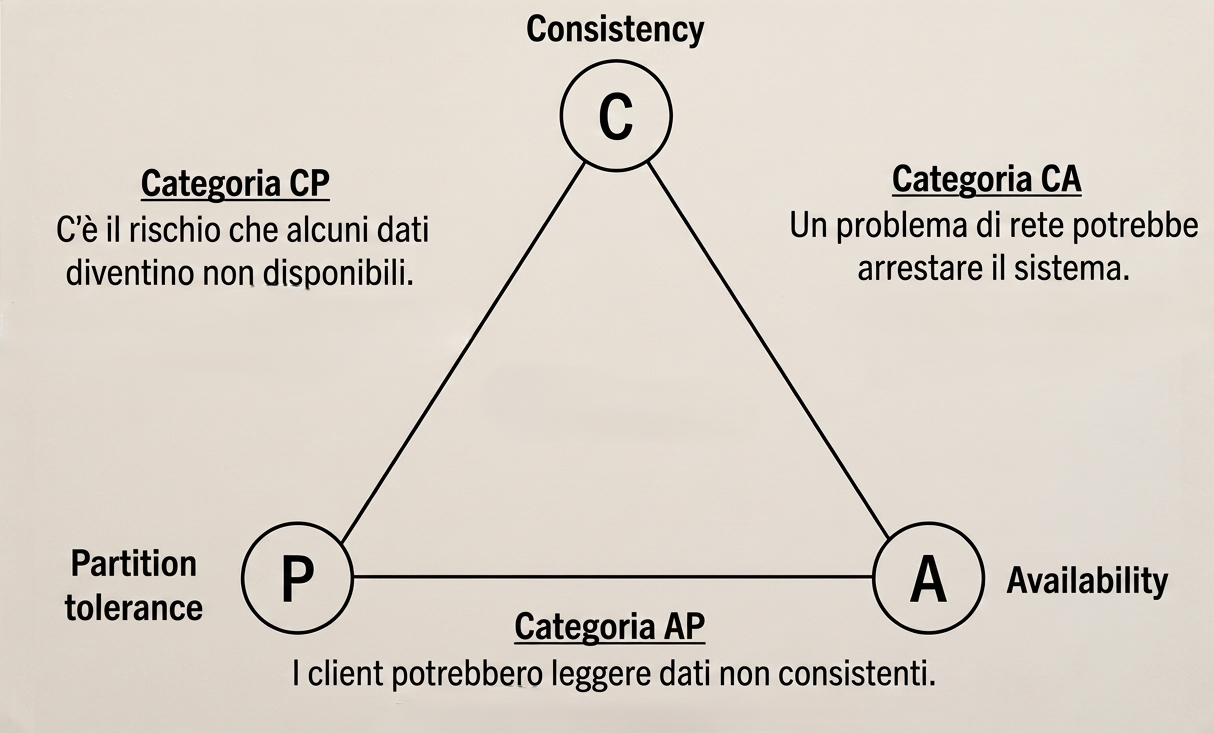
\includegraphics[width=0.8\linewidth]{Figure/CAP_Theoreme.png}
    \caption{Cap theorem}
    \label{f_CAP}
\end{figure}

\noindent
\textbf{Cassandra} viene generalmente classificato come un sistema \textbf{AP} (Availability + Partition Tolerance), infatti privilegia la disponibilità del servizio e la tolleranza alle partizioni, accettando la possibilità di leggere dati non perfettamente aggiornati in alcune condizioni.\newline \newline
Tuttavia, grazie al modello di \textbf{consistenza configurabile} (Tunable Consistency), è possibile modulare il grado di coerenza dei dati definendo opportunamente le politiche di lettura e scrittura. In questo modo il sistema può avvicinarsi a un comportamento di tipo \textbf{CP} (Consistency + Partition Tolerance), a scapito della disponibilità in presenza di condizioni avverse della rete.
In particolare le politiche di lettura e scrittura principali possono essere:

\begin{itemize}
    \item \textbf{ONE:} Basta la conferma di una replica. Massima velocità, ma rischio di leggere dati vecchi.
    \item \textbf{QUORUM:} Richiede la conferma della maggioranza (es. 3 su 5). È il bilanciamento ideale per la maggior parte dei sistemi.
    \item \textbf{ALL:} Richiede la conferma di tutte le repliche. Garantisce consistenza forte, ma riduce la disponibilità (se un nodo è offline, la query fallisce).
\end{itemize}

\subsection{Bloom Filter} \label{s_bloom}

Un \textbf{Bloom filter} è una struttura dati probabilistica utilizzata per verificare l'appartenenza di un elemento a un insieme. È progettato per essere estremamente efficiente in termini di memoria e tempo di risposta, al costo di una possibile presenza di \textbf{falsi positivi}, mentre \textbf{non produce mai falsi negativi}.\newline

\noindent
La struttura si basa su un array di $m$ bit inizialmente impostati a $0$ e su $k$ funzioni di hash indipendenti. Ogni elemento inserito viene elaborato dalle $k$ funzioni di hash, che producono $k$ indici nell’array; i bit corrispondenti a tali posizioni vengono impostati a $1$.\newline

\noindent
La fase di \textbf{query} avviene in modo analogo: l’elemento viene hashato con le stesse $k$ funzioni e si controllano i bit nelle posizioni ottenute. Se \textbf{almeno uno} di questi bit è $0$, l’elemento è \textbf{certamente non presente}. Se invece tutti i bit risultano $1$, l’elemento viene considerato \textbf{potenzialmente presente}, con una certa probabilità di falso positivo.
\noindent
La probabilità di falso positivo dipende principalmente dalla dimensione dell’array $m$, dal numero di elementi inseriti $n$ e dal numero di funzioni di hash $k$: in particolare, all’aumentare di $n$, cresce la saturazione dell’array di bit, aumentando la probabilità di collisioni tra elementi diversi.

\section{Modello dei Dati e Struttura Logica}
A differenza dei database relazionali, Cassandra adotta un approccio \textbf{Wide Column Store}. La gerarchia dei dati è organizzata come segue (un esempio in figura \ref{f_schema}):

\begin{itemize}[leftmargin=*]
    \item \textbf{Keyspace:} Il contenitore di massimo livello (equivalente a un database in SQL). Definisce le impostazioni di replica e il numero di copie dei dati da mantenere nel cluster (si parlerà più approfonditamente di questo nella sezione \ref{s_replicazione}).
    \item \textbf{Tabella (o Column Family):} Definisce lo schema, ovvero colonne e tipi, ma è flessibile e quindi non richiede che ogni riga possieda le medesime colonne.
    \item \textbf{Righe e Colonne:} Ogni riga è identificata da una chiave primaria. Le colonne sono composte da un nome, un tipo e un valore. La flessibilità permette a righe diverse della stessa tabella di avere set di attributi differenti (es. una riga con indirizzo e una senza) senza necessità di valori nulli.

\begin{figure}[H]
    \centering
    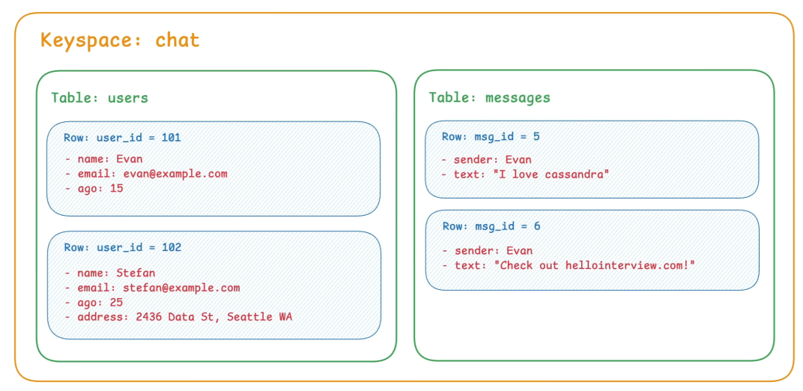
\includegraphics[width=1\linewidth]{Figure/Schema.png}
    \caption{Gerarchia dei componenti}
    \label{f_schema}
\end{figure}
\end{itemize}

\subsection{Modellazione dei Dati Query-Driven} \label{s_denormalization}
In Cassandra, la modellazione dei dati segue un approccio \textbf{Query-Driven}, ovvero conviene progettarla a partire dalle query che l'applicazione dovrà eseguire più frequentemente, anziché dalla rappresentazione delle entità e delle loro relazioni come avviene nei database relazionali.\newline
Per questo motivo, le tabelle vengono create e organizzate in modo da consentire l'accesso diretto ai dati necessari per uno specifico caso d'uso. Ciò porta spesso a una \textbf{denormalizzazione} dei dati, ovvero alla duplicazione controllata delle informazioni in più tabelle per ottimizzare le operazioni di lettura.\newline
Questo approccio riduce la necessità di operazioni costose come \textbf{join} e aggregazioni, che Cassandra non supporta in modo efficiente, garantendo prestazioni elevate e tempi di risposta prevedibili anche su grandi quantità di dati.\newline
Cassandra risulta quindi particolarmente efficiente in sistemi con un \textbf{insieme limitato} e ben definito di \textbf{query}, dove i pattern di accesso ai dati sono noti a priori e i requisiti di scalabilità e disponibilità sono elevati.

\subsection{Meccanismi di Partizionamento e Scalabilità}
La scalabilità orizzontale di Cassandra é ottenuta grazie alla distribuzione dei dati tra i vari nodi, in modo che ognuno gestisca solo una frazione dell'intero dataset, collaborando con gli altri per aumentare la \textbf{availability}.

\subsubsection{La Chiave Primaria} \label{s_primary_key}
La chiave primaria è l'elemento cruciale e si divide in:
\begin{enumerate}
    \item \textbf{Partition Key (Chiave di Partizione):} Determina la posizione fisica dei dati. Tutte le righe con la stessa chiave di partizione risiedono sullo stesso nodo per ottimizzare l'accesso. Ad esempio, usando \texttt{user\_id} come chiave di partizione, tutti i messaggi di un utente specifico saranno raggruppati sullo stesso server.
    \item \textbf{Clustering Key (Chiave di Clustering):} Determina l'ordinamento logico dei dati all'interno della partizione (es. ordinare i messaggi per timestamp).
\end{enumerate}

\subsubsection{Dal Modulo al Consistent Hashing}
Inizialmente, i sistemi distribuiti usavano l'hash della chiave modulo il numero di nodi ($hash \pmod N$). Tuttavia, questo approccio causa uno shuffling massiccio di dati ogni volta che si aggiunge o rimuove un nodo. 
Cassandra risolve il problema con il \textbf{Consistent Hashing}:
\begin{itemize}
    \item I valori di hash sono disposti su un \textbf{anello virtuale}.
    \item Ogni nodo è responsabile di un intervallo di questo anello.
    \item Quando una chiave viene inserita, il sistema calcola l'hash e procede in senso orario sull'anello fino a trovare il nodo giusto.
\end{itemize}

\noindent
L'uso di \textbf{nodi virtuali (vnodes)} permette una distribuzione del carico ancora più uniforme.\newline
Ogni dato è replicato nel nodo relativo all'intervallo calcolato tramite l'hashing ed a \textbf{RF} nodi successivi con r \textbf{replication factor} (si veda sezione \ref{s_replicazione}).
\newline \newline
\noindent
Di seguito una rappresentazione grafica di quanto appena detto:

\begin{figure}[H]
    \centering
    \label{f_nodes}
    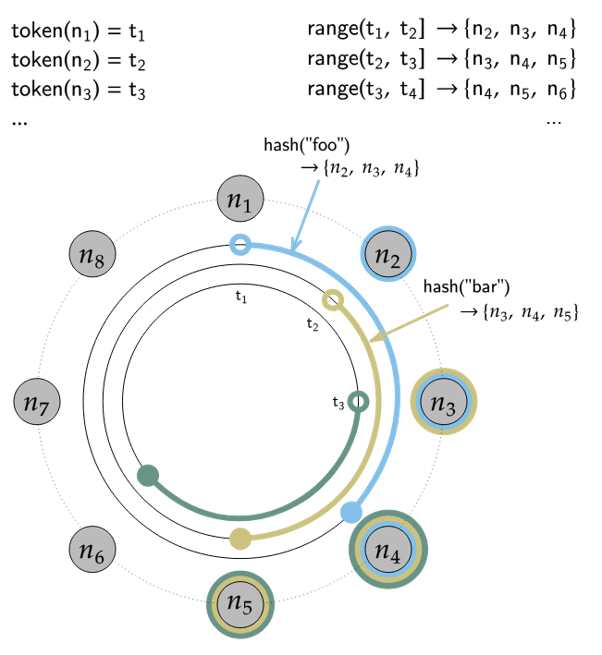
\includegraphics[width=0.7\linewidth]{Figure/Nodes.png}
    \caption{Struttura ad anello dei nodi Cassandra}
\end{figure}

\subsection{Disponibilità e Protocolli Peer-to-Peer}
Cassandra è un sistema \textbf{leaderless}, ovvero senza master: ogni replica è uguale alle altre e ogni nodo può coordinare una richiesta. Per tale ragione sono importanti gli elementi esposti nelle seguenti sezioni (sezioni \ref{s_gossip} e \ref{s_replicazione}).

\subsubsection{Protocollo Gossip} \label{s_gossip}
Per mantenere il cluster sincronizzato senza un coordinatore centrale i nodi comunicano tramite il \textbf{Gossip Protocol}. A intervalli regolari, ogni nodo scambia piccole informazioni con alcuni nodi scelti casualmente riguardo lo stato del cluster (nodi attivi/inattivi, intervalli di dati posseduti, versioni dello schema): questo permette al cluster di auto-gestirsi e di evitare colli di bottiglia o punti di guasto centralizzati.\newline
Questo meccanismo consente anche la \textbf{failure detection}, in particolare rileva l’assenza di comunicazione con altri nodi e li marca prima come \textit{suspect} e poi come \textit{down} se il problema persiste.

\subsubsection{Allineamento repliche}
L'allineamento delle repliche avviene tramite un meccanismo di \textbf{anti-entropy}, basato sull'utilizzo delle \textbf{Merkle Trees}. Tali strutture vengono impiegate durante il processo di \textbf{repair} per confrontare in modo efficiente i dati tra repliche e rilevare eventuali inconsistenze.\newline
Il loro funzionamento si basa sulla costruzione di un albero di hash: i dati vengono suddivisi in intervalli e, per ciascun intervallo, viene calcolato un valore di hash. Gli hash dei nodi foglia vengono poi combinati gerarchicamente fino a ottenere un hash radice. Durante il repair, i nodi confrontano questi hash; se il valore della radice coincide, le repliche sono coerenti, altrimenti il confronto viene approfondito ricorsivamente fino a individuare le differenze.\newline
Di seguito in figura \ref{f_merkleTrees} un esempio di quanto detto:

\begin{figure}[H]
    \centering
    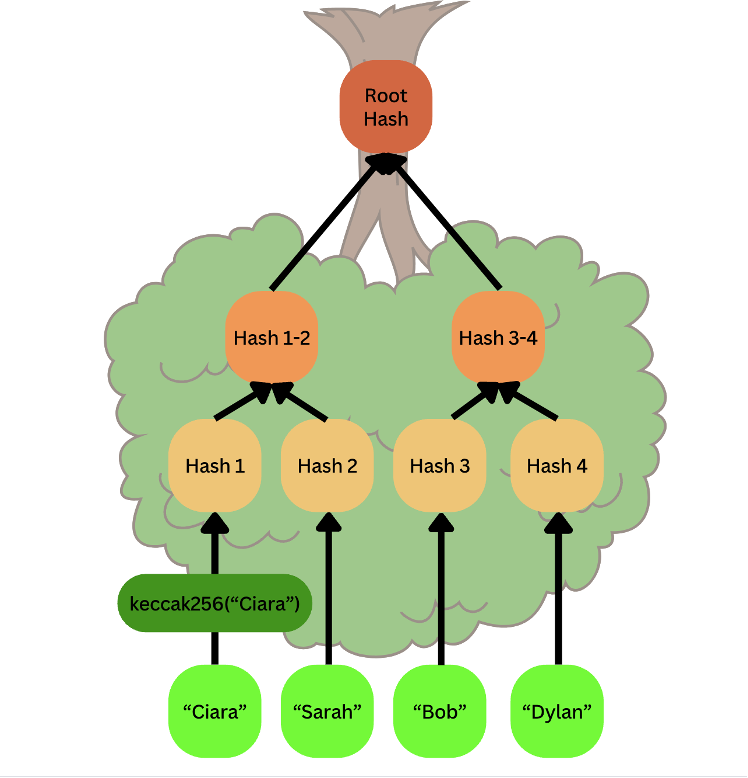
\includegraphics[width=0.6\linewidth]{Figure/MerkleTree.png}
    \caption{Esempio di Merkle-Tree}
    \label{f_merkleTrees}
\end{figure}

\subsubsection{Fattore di Replicazione} \label{s_replicazione}
Il \textbf{Replication Factor (RF)} determina quante copie esistono per ogni dato. Cassandra posiziona le repliche in modo strategico su diversi rack o data center per garantire che, anche in caso di blackout di un intero settore, i dati rimangano accessibili.

\subsection{Architettura di Scrittura e Lettura}

L'architettura descritta segue il modello \textbf{LSM-Tree} (Log-Structured Merge Tree), su cui si basa Cassandra: le scritture vengono prima registrate nel \textbf{Commit Log} e nella \textbf{MemTable} in memoria, per poi essere trasferite su disco in file immutabili chiamati \textbf{SSTable} (Sorted String Tables).\newline
Questo approccio elimina la necessità di aggiornare direttamente i dati su disco, consentendo un throughput di scrittura molto elevato; infatti le SSTable sfruttano l'\textbf{append-only} ovvero i dati non vengono sovrascritti, ma vengono appesi e successivamente consolidati tramite il processo di \textbf{compattazione}.
Quest'ultimo mantiene la versione più recente di ciascun dato in base al timestamp basandosi su oggetti come le \textbf{tombstone}: essi sono dei marcatori di cancellazione che non eliminano immediatamente il dato, ma lo segnalano come rimosso, permettendo la loro eliminazione definitiva solo in seguito durante la compaction.

\subsubsection{Processo di Scrittura}
Cassandra raggiunge velocità di scrittura elevatissime perché evita IO casuali e lock. Il processo è il seguente:
\begin{enumerate}
    \item Il nodo coordinatore riceve la richiesta e la invia alle repliche.
    \item La replica scrive immediatamente nel \textbf{Commit Log} su disco (per la durabilità).
    \item Successivamente scrive nella \textbf{MemTable} in RAM (pattern \textbf{WAL} write-after-log).
    \item Una volta saturata la MemTable, i dati vengono scaricati (flush) asincronamente su disco in file immutabili chiamati \textbf{SS Tables} (Sorted String Tables).
    \item Poiché le SS Table sono immutabili, gli aggiornamenti non sovrascrivono i dati esistenti, ma creano nuove voci unificate poi tramite la \textbf{compattazione} (compaction).
\end{enumerate}

Di seguito uno schema di quanto detto:
\begin{figure}[H]
    \centering
    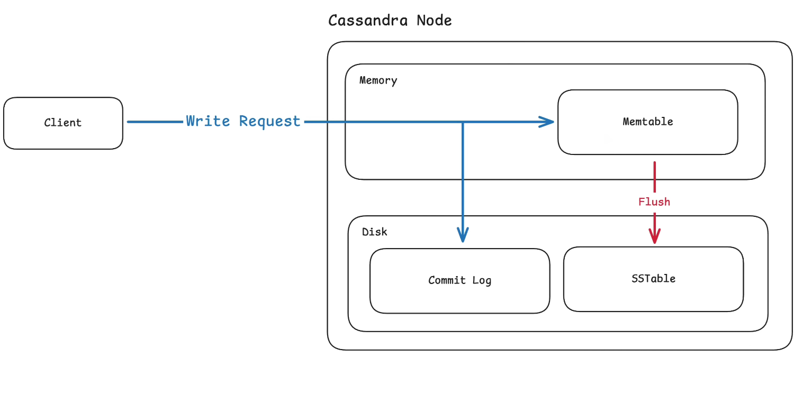
\includegraphics[width=1\linewidth]{Figure/Write.png}
    \caption{Schema di scrittura nel DB}
    \label{f_write}
\end{figure}

\subsubsection{Percorso di Lettura}
La lettura è più complessa: il sistema deve consultare la MemTable e potenzialmente diverse SS Tables. Per mantenere le prestazioni:
\begin{itemize}
    \item Utilizza \textbf{Bloom filter} per escludere file che sicuramente non contengono il dato e indici specifici.
    \newline
    I Bloom filter sono strutture dati \textbf{probabilistiche} che consentono di verificare rapidamente se un elemento non è presente in un insieme: possono generare falsi positivi ma non falsi negativi. Per una descrizione più dettagliata vedere la sezione \ref{s_bloom}.
    \item Se le repliche restituiscono dati diversi, il coordinatore sceglie il valore con il timestamp più recente.
    \item Viene avviato un \textbf{Read Repair} in background per aggiornare le repliche che avevano dati obsoleti.
\end{itemize}

Di seguito uno schema di quanto detto:
\begin{figure}[H]
    \centering
    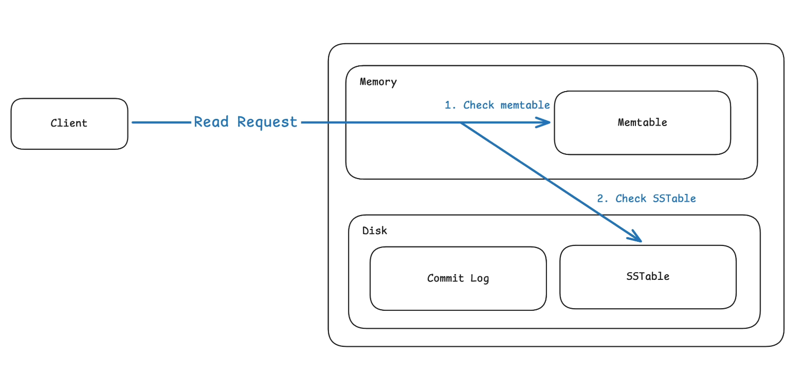
\includegraphics[width=1\linewidth]{Figure/Read.png}
    \caption{Schema di lettura nel DB}
    \label{f_write}
\end{figure}

\section{Sviluppo e Progettazione Database}

\subsection{Dominio applicativo}
Il dominio riguarda la progettazione e gestione di un \textbf{social network} distribuito (Twitter-like), in cui gli utenti possono registrarsi, creare e condividere post anche con contenuti multimediali, seguire altri utenti e consultare un feed personalizzato dei contenuti pubblicati dalle persone che seguono.\newline\newline
I \textbf{contenuti multimediali} non vengono realmente memorizzati nel database Cassandra, ma sono rappresentati tramite generazioni di bit casuali o link fittizi, con lo scopo di simulare la presenza di foto e video che, in un’architettura reale, sarebbero tipicamente archiviati in sistemi esterni dedicati allo storage distribuito.\newline\newline
Un \textbf{utente} è definito da \textit{username}, \textit{email}, \textit{password} hashata, \textit{nome}, \textit{cognome} e un'eventuale \textit{immagine profilo}.
Un \textbf{post} è definito dallo \textit{username} (ovvero l'utente che lo ha pubblicato), da un \textit{id} (generato a partire dall'username e dal timestamp), dal \textit{testo} e possibilmente una \textit{risorsa multimediale} e una \textit{location}. Inoltre sono definite le tabelle \textbf{followers\_by\_user} e \textbf{following\_by\_user} per tracciare le relazioni tra utenti.

\subsection{Architettura codice}
Per analizzare il comportamento di Cassandra sono stati simulati $n$ nodi, ciascuno eseguito all'interno di un diverso \textbf{Container Docker}. Questo ci consente un possibile incremento progressivo del numero di nodi, con l'aspettativa che le prestazioni del sistema crescano in modo approssimativamente lineare.
\newline\newline
Successivamente sono state eseguite anche prove di \textbf{fault tolerance}, simulando la caduta di uno o più nodi al fine di verificare la robustezza del sistema e la sua capacità di continuare a operare correttamente.
\newline\newline
Le componenti principali del codice sono:
\begin{itemize}
    \item \texttt{dbLogic.py}: Gestisce la logica del database e le operazioni correlate per il suo setup
    \item \texttt{docker-compose.yml}: avvia un cluster Cassandra a \textit{n} nodi in Docker, configurando un cluster chiamato “CassandraCluster” con replica tra nodi, persistenza dei dati su volumi separati e controlli di healthcheck e dipendenze di avvio tra i servizi
    \item \texttt{schema.cql}: definisce il keyspace e le tabelle del database, modellando utenti, post, feed e relazioni di follower/following ottimizzati per query specifiche: profilo, timeline e rete sociale
    \item \texttt{workload*.py}: si occupa del popolamento dei dati e della simulazione di operazioni su diverse configurazioni del sistema, al fine di riprodurre scenari realistici di utilizzo.
\end{itemize}

\noindent
Nelle sezioni seguenti saranno analizzati più approfonditamente alcuni componenti di interesse.

\subsection{schema.cql}
Definisce un keyspace Cassandra denominato \texttt{"network\_giustino"}, al suo interno si può configurare la strategia di replica ed il fattore di replica (visto nella seione \ref{s_replicazione}).\newline\newline
All'interno del keyspace vengono definite diverse tabelle per supportare le funzionalità principali di un social network. La tabella \texttt{users} memorizza le informazioni degli utenti, identificati univocamente tramite \texttt{username}, includendo un'immagine profilo salvata come blob e informazioni anagrafiche come nome, cognome, l’indirizzo email, la password sotto forma di hash implementato con SHA256.\newline\newline
La tabella \texttt{posts\_by\_user} modella i post degli utenti, utilizzando una chiave di partizione basata su \texttt{username} e una chiave di clustering \texttt{post\_id} di tipo \texttt{timeuuid} ordinata in modo decrescente per consentire il recupero rapido dei post più recenti (si veda il significato delle chiavi alla sezione \ref{s_primary_key}).\newline
La tabella \texttt{home\_feed} è progettata per ottimizzare la lettura del feed personale, precomputando i contenuti visibili a ciascun utente e ordinandoli per data.\newline
Le relazioni sociali sono gestite tramite due tabelle denormalizzate: \texttt{following\_by\_user}, che memorizza gli utenti seguiti da ciascun utente, e \texttt{followers\_by\_user}, che rappresenta invece gli utenti che seguono un determinato profilo.\newline\newline
Questa struttura segue il paradigma di Cassandra basato sulla denormalizzazione e sulla progettazione orientata alle query (si veda sezione \ref{s_denormalization} per più dettagli).

\subsection{docker-compose.yml}
È un file di configurazione e definisce i nodi del cluster Cassandra con l’obiettivo di simulare il sistema in locale.\newline
Tutti i nodi utilizzano l’immagine ufficiale \texttt{cassandra:4.1} e appartengono allo stesso cluster logico denominato \texttt{CassandraCluster}, garantendo così la possibilità di replicare dati e testare scenari di consistenza e tolleranza ai guasti.\newline\newline
\noindent
Il primo nodo funge da \textit{seed node}, ovvero punto di riferimento iniziale per la formazione del cluster, mentre gli altri nodi si collegano ad esso tramite la variabile \texttt{CASSANDRA\_SEEDS}. La configurazione utilizza lo \texttt{SimpleSnitch}, adatta a deployment single-datacenter, coerente con un ambiente di sviluppo.\newline\newline
\noindent
Un aspetto rilevante è la gestione delle risorse JVM, dove vengono impostati esplicitamente i limiti di heap (\texttt{MAX\_HEAP\_SIZE} e \texttt{HEAP\_NEWSIZE}) per ottimizzare le prestazioni in un contesto containerizzato. Inoltre, sul primo nodo viene abilitato l’accesso JMX remoto tramite \texttt{LOCAL\_JMX=no} e parametri JVM aggiuntivi, permettendo il monitoraggio del cluster.\newline\newline
\noindent
Per garantire una corretta inizializzazione, i nodi sono collegati tramite \texttt{depends\_on} e \texttt{healthcheck}, che verificano la disponibilità del servizio Cassandra tramite comandi CQL prima di avviare i nodi successivi.\newline\newline
\noindent
Vengono inoltre esposte le porte \texttt{9042} e \texttt{7199}: la prima è utilizzata da Cassandra per le connessioni client tramite protocollo CQL, mentre la seconda è dedicata al monitoraggio del sistema attraverso JMX, consentendo l’accesso a metriche e strumenti di analisi.\newline
\underline{Osservazione:} tramite il comando "\texttt{jconsole}" e collegandosi a "\texttt{localhost:7199}" si otterrà una visualizzazione grafica delle performance\newline\newline
\noindent
Infine, vengono definiti volumi persistenti separati per ciascun nodo, assicurando la durabilità dei dati anche in caso di riavvio dei container.

\subsection{dbLogic.py} \label{s_dbLogic}
Implementa la logica applicativa: la classe principale \texttt{DBLogic} gestisce la connessione al cluster, la configurazione del keyspace e la preparazione delle query CQL, ottimizzando le prestazioni tramite l’uso di \textbf{prepared statements}, ovvero query che vengono precompilate e analizzate una sola volta dal database. In fase di esecuzione, tali query ricevono esclusivamente i parametri dinamici, evitando così la ripetizione delle operazioni di parsing e pianificazione dell’esecuzione ad ogni richiesta e riducendo significativamente l’overhead computazionale.\newline\newline
\noindent
Una parte centrale del sistema è la generazione di dati realistici, realizzata tramite la libreria \texttt{Faker}. Vengono creati utenti, post e relazioni sociali (following/followers) con \textbf{distribuzioni probabilistiche} che simulano comportamenti realistici, come il numero variabile di post per utente e la presenza opzionale di contenuti multimediali (per esempio un post deve avere un testo mentre una risorsa audio/video non é obbligatoria).\newline
La libreria \texttt{Faker} può generare potenziali duplicati, poiché attinge da un insieme limitato di dati predefiniti. Per questo motivo è stato necessario introdurre una struttura dati di tipo \texttt{set}, utilizzata per garantire l’unicità degli identificativi (in particolare degli username), evitando così inserimenti duplicati e mantenendo l’integrità delle chiavi primarie nel database.\newline\newline
\noindent
Per migliorare le prestazioni in fase di popolamento del database, il codice utilizza \textbf{esecuzioni concorrenti} tramite il metodo del driver Python di Cassandra \newline \texttt{execute\_concurrent\_with\_args}, riducendo significativamente il tempo necessario per inserire grandi quantità di dati: infatti, per inserimenti con più di 15 elementi (parametro opportunamente scelto), l'utilizzo del metodo consente di eseguire più operazioni in parallelo anziché in modo sequenziale, in questo modo si riduce il tempo complessivo di esecuzione e si migliora l'utilizzo delle risorse di rete e del client.\newline\newline
\noindent
Inoltre, viene implementata una strategia di \textbf{fan-out on write} per la home feed, precomputando le timeline degli utenti in base ai loro follower (maggiorni dettagli nella sezione \ref{s_workload}).\newline\newline
\noindent
La logica include anche la gestione delle relazioni sociali attraverso tabelle denormalizzate, coerenti con il modello di Cassandra, aggiornate simultaneamente per garantire coerenza tra viste complementari (following e followers).\newline\newline
\noindent
Infine, sono presenti funzioni di inserimento singolo e batch per utenti, post e relazioni, che permettono sia test mirati sia generazione massiva di dati per benchmarking del sistema.

\subsection{workload*.py} \label{s_workload}
Implementa gli \textbf{scenari} di utilizzo volti a simulare il comportamento realistico degli utenti di un social network e a misurare le prestazioni del cluster Cassandra in termini di throughput e latenza in varie situazioni.\newline
Generalmente per ogni scenario viene inizializzato il database con un insieme di utenti, post e relazioni sociali generate automaticamente. Solo in alcuni scenari il sistema avvia più \textbf{thread}, per simulare anche la \textbf{concorrenza}.\newline\newline
\noindent
La casualità é affidata all'esecuzione ciclica delle principali operazioni tipiche di un social network secondo una \textbf{distribuzione probabilistica}: consultazione della propria home feed (50\% delle operazioni), creazione di una nuova relazione di follow (30\%) oppure pubblicazione di un post (20\%). In questo modo il benchmark riproduce un carico misto di letture e scritture, più vicino a uno scenario reale rispetto a test sintetici basati su una singola tipologia di query.\newline\newline
\noindent
Particolare attenzione è dedicata alla simulazione della strategia \textbf{fan-out on write}, come detto nella sezione \ref{s_dbLogic}. Quando un utente pubblica un nuovo contenuto, il sistema recupera dal database l'elenco reale dei suoi follower e inserisce immediatamente una copia del post nella home feed di ciascuno di essi. Questa scelta consente di valutare il costo computazionale della propagazione dei contenuti in fase di scrittura, approccio comunemente adottato nei social network per velocizzare le successive operazioni di lettura.\newline\newline
\noindent
Al termine dell'esecuzione vengono raccolte e analizzate le \textbf{metriche} principali del sistema, tra cui il numero totale di operazioni completate, il throughput espresso in operazioni al secondo e la latenza media delle richieste. Tali misure consentono di valutare il comportamento del cluster Cassandra sotto un carico concorrente e di confrontare l'impatto delle diverse configurazioni o strategie di modellazione dei dati.\newline\newline
\noindent
Questo componente gestisce le interazioni effettive con il database e le operazioni su di esso; non è quindi costituito da una singola classe, ma da un insieme di classi, come illustrato di seguito:

\begin{itemize}
    \item \texttt{workloadBase}: carica 1000 utenti, 50 dei quali effettuano ogni 0.5 secondi delle operazioni casuali. Questo componente utilizza 50 \textbf{thread} per simulare la concorrenza nelle operazioni
    \item \texttt{workloadConsistency}: carica 5000 utenti e fa 1000 operazioni casuali senza concorrenza
    \item \texttt{workloadPayload}: carica 1000 utenti di cui 500 caricano un post con dei file multimediali di 1 \textit{kByte} e 500 caricano dei file multimediali di 100 \textit{kByte}. Questo scenario serve appositamente per testare le performance a differenza di payload dei post
    \item \texttt{workloadReadMiss}: carica 100 utenti e fa query base su utenti esistenti e non esistenti per testare le performance relative a \textbf{hit} e \textbf{miss} nel database
    \item \texttt{workloadStressTest}: carica 25 utenti in concorrenza; lancia quindi 25 thread che effettuano 100 caricamenti ognuno di post in parallelo per testare una situazione di stress
    \item \texttt{workloadFaultTolerance}: Si simula il carico di un utente che esegue un’operazione al secondo, testando il sistema in diverse configurazioni del \textbf{consistency level} (si veda Sezione \ref{s_cap}). Inoltre, nel presente workload è stata valutata la \textbf{caduta dei nodi}: per un cluster di \( n \) nodi, sono state eseguite 10 richieste, dopodiché è stato fatto fallire un nodo; successivamente sono state inviate altre 10 richieste e si è proceduto alla caduta di un ulteriore nodo. Tale processo è stato ripetuto per \( n-1 \) iterazioni, fino al guasto progressivo di tutti i nodi tranne uno. Questa procedura è stata eseguita per ciascun consistency level considerato.
\end{itemize}

\section{Performance in Situazioni Stabili}

\section{Performance con Caduta Nodi}

\section{How to Run}
L'intero progetto è sviluppato in Python e richiede l'installazione di alcune dipendenze esterne, in particolare le librerie \texttt{cassandra-driver} e \texttt{Faker}. Per una corretta gestione delle dipendenze è consigliato creare un ambiente virtuale dedicato (\texttt{venv}), in modo da isolare le librerie del progetto dal resto del sistema.\newline\newline
\noindent
La creazione dell'ambiente virtuale può essere effettuata tramite il comando:

\texttt{python -m venv .venv}

\vspace{0.5cm}
\noindent
Successivamente, l'ambiente può essere attivato con:

\textbf{Windows:} \texttt{.venv\textbackslash Scripts\textbackslash activate}

\textbf{Linux/macOS:} \texttt{source .venv/bin/activate}

\vspace{0.5cm}
\noindent
Una volta attivato l'ambiente virtuale, è possibile installare tutte le dipendenze richieste spostandosi nella cartella del progetto ed eseguendo:

\texttt{pip install -r requirements.txt}

\vspace{0.5cm}
\noindent
In alternativa, le librerie possono essere installate singolarmente:

\texttt{pip install cassandra-driver}\newline

\texttt{pip install Faker}

\subsection{Avvio del cluster Cassandra tramite Docker}

Per eseguire il cluster Cassandra è necessario aver installato Docker e Docker Compose.\newline
L'avvio dei container può essere effettuato tramite:

\texttt{docker compose up -d}

\vspace{0.5cm}
\noindent
Una volta avviato il cluster, alcuni comandi utili per monitorarne lo stato sono:

\textbf{Verifica stato nodi}:\\
\hspace*{1cm}\texttt{sudo docker exec -it cassandra-node1 nodetool status}

\textbf{Visualizzazione topologia cluster}:\\
\hspace*{1cm}\texttt{sudo docker exec -it cassandra-node1 nodetool describecluster}

\vspace{0.5cm}
\noindent
Nel caso in cui un nodo non venga avviato correttamente, è possibile riavviarlo mediante:

\texttt{sudo docker restart cassandra-<nome\_nodo>}

\underline{Oss:} Su sistemi Windows il prefisso \texttt{sudo} può essere omesso

\subsection{Caricamento dello schema}

Dopo l'avvio del cluster è necessario caricare lo schema Cassandra definito nel\newline
file \texttt{schema.cql}.

\textbf{Windows}:\\
\hspace*{1cm}\texttt{Get-Content schema.cql | docker exec -i cassandra-node1 cqlsh}

\textbf{Linux/macOS}:\\
\hspace*{1cm}\texttt{sudo docker exec -i cassandra-node1 cqlsh < schema.cql}

\subsection{Popolamento del database}

Una volta creato lo schema, il database può essere popolato con dati sintetici eseguendo lo script Python dedicato:

\texttt{python3 dbLogic.py}

\subsection{Accesso alla shell CQL}

Per interagire direttamente con Cassandra ed eseguire query manuali è possibile accedere alla shell CQL tramite:

\texttt{sudo docker exec -it cassandra-node1 cqlsh}

\vspace{0.5cm}
\noindent
Ad esempio, una volta aperta la shell, è possibile interrogare la tabella degli utenti mediante:

\texttt{SELECT username, email, first\_name, last\_name}\newline

\texttt{FROM users;}

\subsection{Gestione dei container}

Per arrestare temporaneamente i container mantenendo i volumi persistenti:

\texttt{sudo docker compose stop}

\vspace{0.5cm}
\noindent
Per riavviare i container precedentemente arrestati:

\texttt{sudo docker compose start}

\vspace{0.5cm}
\noindent
Per eliminare i container mantenendo i volumi:

\texttt{sudo docker compose down}

\vspace{0.5cm}
\noindent
Per eliminare sia i container sia i volumi associati:

\texttt{sudo docker compose down -v}

\section{Conclusioni}

\end{document}